\iffalse
3. Teori
Här kan ett videoprojekt beskriva videoformatet, ett MIDI-projekt redogöra för MIDI-standarden ...
\fi


\section{Teori}
	Här gås teorietiska bakgrunderna för tekniken som använts i projektet.

\subsection{VGA}
	VGA (Video Graphics Array) introducerades först och främst på en IBM\circledR PS/2 dator i 1987 och en CRT-skärm. På Nexys 3 finns VGA, och därför användes detta till projektet. VGA standarden använder sig av en amplitudmodulerade rörliga elektroner för att visa en bild på monitorn. Standarden för visning och svepande av elektronstråle kräver en bra synkroniseringen. Detta för att den elektroniska kanonen som projicerar bilen måste hinna klart med alla rader innan bilden uppdateras. För att kanonen ska rikta om sig finns blankområdet, som ligger utanför det synliga fältet. Den tiden ger möjlighet för kanonen att ställa om sig till nästa rad. 
	Standarden har en feltolerans på $\pm0.5\%$, klockan i projektet skalas ner till så nära som möjligt för att kunna ge en hyfsad rätt frekvens \cite{vgasite}. I figur \ref{fig:vgateori} kan en god översikt ges av VGA-timingsen.


	\begin{center}
		\begin{figure}[H]
    		\centering
			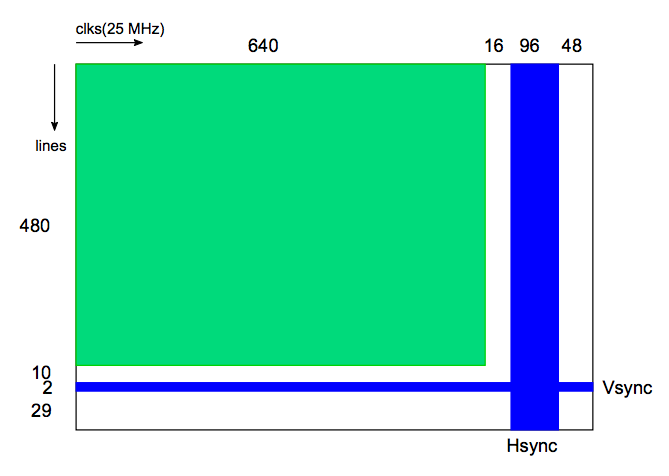
\includegraphics[scale=0.50]{../grafik/rapport-vgateori.png}
			\caption{VGA-timings \cite{vgapic}}
			\label{fig:vgateori}
		\end{figure}
	\end{center}


\subsection{Analog till digital konvertering}
	En analog till digital konvertering går ut på kvantisera de analoga signalerna exempelvis en elektrisk spänning till ett digitalt värde. Det analoga värdet kan anta vilka värden som helst, men det digitala enbart kan anta 0 eller 1. För att skapa en digital version behövs flera värden mätas och omvandlas. Vid en bestämd frekvens tas ett värde ut från den analoga signalen, detta kallas ett sampel. För att det inte ska bli någon interfereras läggs A/D-omvanldaren i ett \"sample-and-hold\" läge, och det utvalda värden kan därefter omvandlas. \cite{analogsite}.
	De fel man kan upptäcka på en A/D-omvandlare är ofta samma som felen som uppträder för en D/A-omvandlare. Vilka är:
	\begin{enumerate}
		\item Linjäritetsfel, kan ges upphov till av tillverkningstoleransen av motstånden.
		\item Offsetfel, balansen för nästkommande förstärkare är ur fas.
		\item Skalfel, en frekvens som inte är linjär.
	\end{enumerate}
	\cite{tsea82_2014}

	Här är ett exempel på hur en analog signals kurva ser ut, samt med alla sampel inritade.

	\begin{center}
		\begin{figure}[H]
    		\centering
			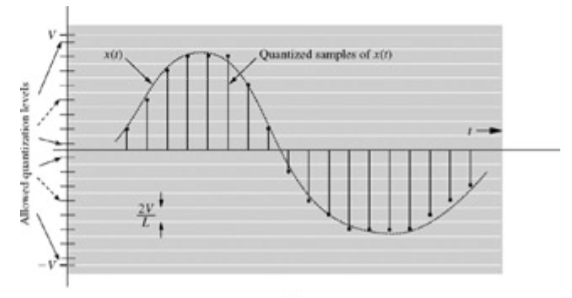
\includegraphics[scale=0.50]{../grafik/adc.png}
			\caption{VGA-timings \cite{adcpic}}
			\label{fig:adcteori}
		\end{figure}
	\end{center}